\documentclass{article}
    \title{\textbf{Machine Learning Project}}
    \author{Fabio Massimo Ercoli}
    \date{July 2024}
    \usepackage{amsmath,algpseudocode}
    \algdef{SE}[EVENT]{Event}{EndEvent}[1]{\textbf{upon event}\ #1\ \algorithmicdo}{\algorithmicend\ \textbf{event}}%
	  \algtext*{EndEvent}
    \usepackage{graphicx}
\begin{document}

\maketitle

\section{Introduction}

We're presenting two prossible Q-learning implementation approaches:
\begin{itemize}
  \item Tabular based. Implemented using a numpy dictonary.
  \item Neural network based. Also known as Deep Queue Network (DQN).
\end{itemize}

\section{Tabular Q-Learning}

\subsection{Running the project}

To trigger the learning process run from the \emph{machine-learning-project} directory the following code:

\begin{verbatim}
python qlearn-app.py
\end{verbatim}

You should see a message similar to the following:

\begin{verbatim}
observation space Discrete(500)
action space Discrete(6)
avg return before learning -92.98608555399927
avg return after learning 2.5552244875845997
\end{verbatim}

The observation and the action space description is related to the \emph{Gymnasium} environment we used to train and test our agent, 
that is the \emph{Taxi-v3 environment}\footnote[1]{$https://gymnasium.farama.org/environments/toy_text/taxi$} that has 500 discrete possible states and 6 possible actions.

The \emph{avg return} is the average of the score gained rolling out a series of episodes.
In the case of this project 5 episodes are executed before the training and 20 after the training.
The expectation is that the agent can get a better score after we properly trained it.

An episod starts from the initial state and ends in case of a termination state is reached or is trunkated since the \textbf{max episode steps} value is reached.

This is the first value we can change to tune the lerning, in general this value should be great enough to allow the agent to learn and to rollout correctly the strategy it learned.
We decide to increase it from 200, that is the default, to 500 and this change seems to provided better performance to the learning.

How can we evaluate the goodneed of the learning? In this case we simpy compare the average score for an episode perfomed using a random strategy (before to learn)
with the average score obtanied after the learn.

\subsection{The rollout and the score}

The score is a crucial concept, since the learning activity is entirly oriented to maximaize this value.

The score is the summation of all the reward we get from the environment every time we execute an action (notice that can be negative or positive),
multiplied by the \textbf{discount factor} $\gamma$.

The meaning of this value is to promote not only the rewards collected, but also the speed with which we get them.
This is another value that we need to balance, since if it is too low, we can penalize the learning of long term goals.

The score depends on the actions the agent chooses, those are randomly selected before the training 
and after the training they are chosen according to the learned policy.

The rollout procedure will collect the score for each epoch, applying the current discount factor to the reward.
The score is averaged and retured to the caller.

\subsection{The learning and the Q function}

The output of the learning is a policy to choose for any given state (observation)\footnote[2]{
In the context of this project that state is always fully observable, so we will use the term state and observation interchangebly} 
an action among all possible actions to apply.
The Q function associate to a given state and a given action the expected total score of taking the action in the state 
and then continue to choose optimally the futher actions.
So we can use the Q function to choose the policy as the action that maximaizes the expected total score.

We call it the \emph{greedy policy}, since it maximaizes the expected score not conisidering the fact that unexplored paths may
possibly lead to even greater scores, improving the Q function.
At the begin of the learning we want always to apply a random strategy to learn as much as possible ($\epsilon = 0$).
At the end of the learning on the other hand we want to exploit the knowledge we've acquired to perfectionate the policies on areas
that we already know to be good ($\epsilon \approx 1$).
In this project we use a linear decay from 0 to 1 of the \textbf{greedy factor} $\epsilon$ for the learning.
Other decay functions of course are possible.

How should the learning last for? In this project the learning finishes as soon as we run a number of actions
equals to the \textbf{learning steps}. In this project we set this value to 200,000.

The last crucial setting we present in this chapter is the \textbf{learning rate} $\alpha$\textsubscript{0}.
The Q function is updated for supporting the indeterministic environments according to the formula:

\begin{equation}
  Q(s,a) = (1 - \alpha) Q(s,a) + \alpha [r + \gamma \max\textsubscript{a'} (Q(s',a'))]
\end{equation}

Where s' is the state we get from s applying the action a, 
and the $\max (Q(s',a'))$ is calculated among all the possible action a' executable from s'.

\subsection{The tabular approach}

In this implementation the values for the Q function are stored as table items,
in particular in order to represent only the subset of state we're interested in we use 
in this project a dictonary (instead of an array).

This means that every time we update an entry on the Q function we operate on a discrete value of the
observation and on a discrete value of the action.

Thus in order to support with this approach continuous environment,
we need first to apply a discretize of the state (and/or the action).

Figure 1 \ref{fig:qlearning} presents the graph of the sum of the total rewards (not discounted) per episode get during the learning process.
You can see the improvement given by the fact that the:

\begin{itemize}
  \item Moving forward the actions are increasingly greedy and less random.
  \item The agent is actually learning how to act better.
\end{itemize}

\begin{figure}
  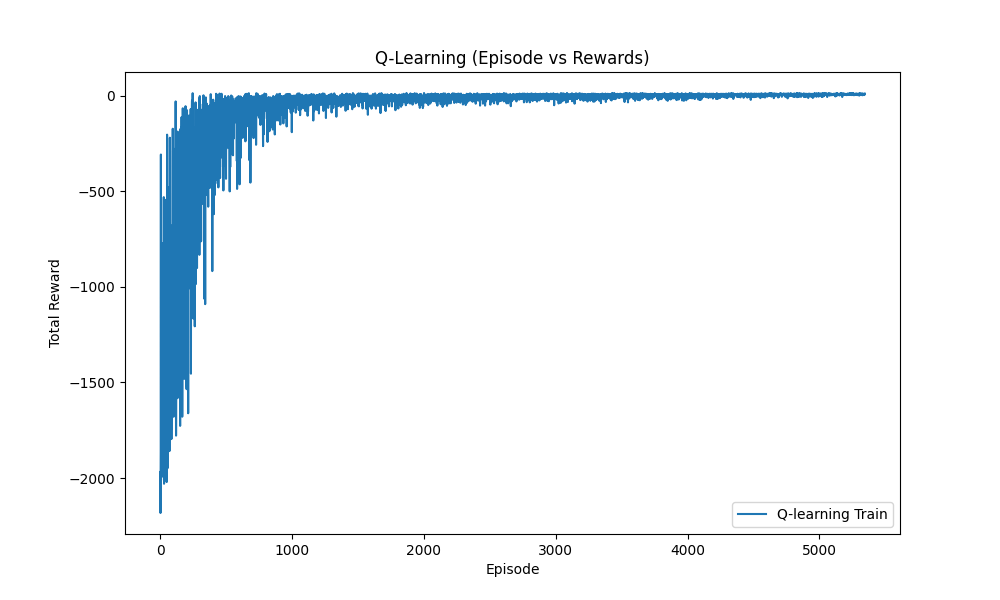
\includegraphics[width=\linewidth]{qlearning.png}
  \caption{Q-Learning}
  \label{fig:qlearning}
\end{figure}

\section{Deep Q-Learning}

\subsection{Running the project}

To trigger the learning process run from the \emph{machine-learning-project} directory the following code:

\begin{verbatim}
python dqn-app.py
\end{verbatim}

\subsection{Network design}

A completely different way to represent the Q function is to use a neural network to denote it.
In this case the result of the learning will be the training of the network.

In the implementation provided by this project the neural network has been designed to have:
\begin{itemize}
  \item One input node for each state value, in the \emph{input layer}.
  \item One output node for each action that can be performed, in the \emph{output layer}.
  \item Two middle layers of size 24 each.
\end{itemize}

In the output layer we use a linear function (returning any real value) for each action,
since the result of $Q(s,a)$ can assume any real value.

In the middle layers we use the \emph{relu} activation function, that provides the fundamental 
non linear property to the network.

The network is dense, so the nodes between two adjacent layers are fully connected.

\subsection{Mini batch approach}

Each time we execute a step among the environment we collect the tuple:

\begin{verbatim}
  < state, action, reward, next_state, done >
\end{verbatim}

in the \emph{replay buffer}.
We want to keep only the last \emph{50,000} events, so we implemented it as bounded deque.

We train the network using a minibatch strategy that consists
in randomly selecting a fixed size batch of events,
in our case \emph{128}, from the replay buffer and use it to train the network,
as a unit training step.

The benefiths of this approach are that:

\begin{itemize}
  \item We save a lot computational resources, 
  since we processes arrays of events, basically a matrix, at each $model.fit$ invocation.
  \item The fact that every time we select a random subset of events 
  to train the network allows to implement the stocastic gradient discend, that allows
  to be not trapped in a local minimum when we compute the loss function.
\end{itemize}

\subsection{Policy and target networks}

In this project we used two networks, having the same architecture but different weight:

\begin{itemize}
  \item A policy network, also called the main network:
  \begin{itemize}
    \item{Updated every very few steps (4 in our project)}
  \end{itemize}   
  \item A target network:
  \begin{itemize}
    \item{Synchronized each time only after we execute 10 episodes}
    \item{Used to compute the $\max\textsubscript{a'} (Q(s',a'))$, when we calculate a new Q value}
  \end{itemize} 
\end{itemize}

This strategy leads to more stability in the learning process.

\subsection{Difference with the tabular approach}

There are two main difference, compared with the tabular Q-learning:

\begin{itemize}
  \item{The Q function values are approximated, not exact}
  \item{With the DQN we can train agent in environments having a countinous state values}
\end{itemize}

On the other hand other aspects are in common between the two approaches, such as
the formula to compute the new $Q(s,a)$ value, or the application of the epsilon strategy
to choose between the exploration action or a greedy (policy) action during the learning process.

\subsection{DQN project models}

I tried to steal some ideas from some opensource preexisting projects from the web.
In particular from \emph{minDQL}\footnote{minDQL https://github.com/mswang12/minDQN} on which I also to contribute with 
a \emph{pull request}\footnote{My pull request: https://github.com/mswang12/minDQN/pull/9} 
to aling the source code with the last versions of TensorFlow and Gymnasium.

The stealed ideas was:

\begin{itemize}
  \item{To use two neural networks instead of one to stabilize the learning (see Policy and target networks)}
  \item{To run the replay procedure from the replay buffer not at after each step to make the learning faster}
  \item{To train the network on an array of Q values instead of on each at the time
  \footnote{This is was also mentioned in the course, but the project helped me in having a reference implementation for the minibatch}}
\end{itemize}

And I applied them to my project.

\subsection{DQL variables}

\begin{tabular}{ c c c }
  learning rate & $\alpha\textsubscript{0}$ & 0.1 \\
  exploration / greedy & $\epsilon$ & linar decay from 0 to 1 \\
  discounting factor & $\gamma$ & 0.95 \\  
  replay buffer size & - & 50,000 \\
  min replay buffer size & - & 1,000 \\
  mini batch size & - & 128 \\
  train episodes & - & 300 \\
  steps to update policy model & - & 4 \\
  steps to update target model & - & 100  \\
  max episode steps & - & 500
 \end{tabular}

\end{document}